\documentclass[tikz,border=4pt]{standalone}
\usepackage{fontspec}\setmainfont{TeX Gyre Pagella}
\hyphenpenalty=10000\exhyphenpenalty=10000
\usetikzlibrary{arrows.meta,positioning,calc,fit,backgrounds}
\definecolor{acc}{HTML}{1F5FBF}\definecolor{gry}{HTML}{8A8A8A}\definecolor{lg}{HTML}{C8C8C8}\definecolor{fillacc}{HTML}{E6EEFA}\definecolor{fillg}{HTML}{F1F1F1}\definecolor{ink}{HTML}{222222}
\tikzset{box/.style={draw=gry,rounded corners=3pt,line width=0.6pt,align=center,inner sep=5pt,font=\small},
 hl/.style={box,draw=acc,fill=fillacc,line width=0.9pt},dbox/.style={box,dash pattern=on 3pt off 2pt},
 arr/.style={-{Stealth[length=5pt]},line width=0.6pt,draw=gry},aarr/.style={-{Stealth[length=5pt]},line width=0.9pt,draw=acc}}

\begin{document}
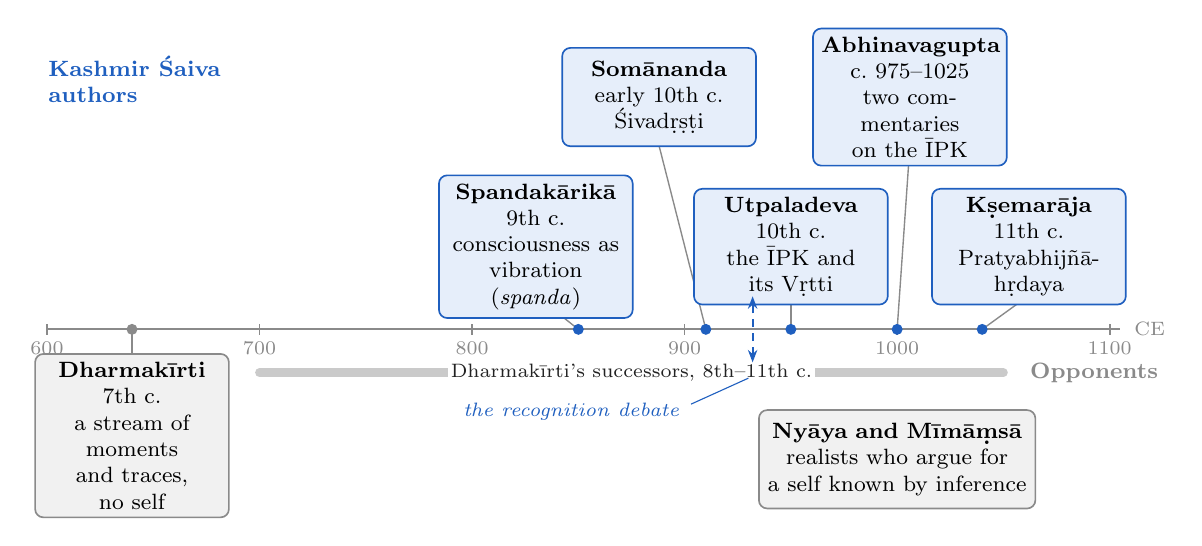
\begin{tikzpicture}[x=0.027cm,y=1cm,
  ev/.style={box,text width=2.25cm,inner sep=3pt,font=\footnotesize,minimum height=1.25cm},
  sv/.style={ev,draw=acc,fill=fillacc},
  bv/.style={ev,fill=fillg},
  tick/.style={gry,line width=0.5pt},
  dot/.style={circle,inner sep=1.4pt,fill=#1}]
% axis (years CE; origin 600)
\draw[gry,line width=0.7pt] (0,0) -- (505,0);
\foreach \c in {600,700,800,900,1000,1100}{
  \draw[gry,line width=0.6pt] ({\c-600},-0.07) -- ({\c-600},0.07);
  \node[font=\scriptsize,text=gry,fill=white,inner sep=1pt] at ({\c-600},-0.24) {\c};}
\node[font=\scriptsize,text=gry,anchor=west] at (507,0) {CE};
% lane titles
\node[font=\footnotesize\bfseries,text=acc,anchor=north west,align=left] at (-4,3.6) {Kashmir Śaiva\\authors};
\node[font=\footnotesize\bfseries,text=gry,anchor=west] at (458,-0.55) {Opponents};
% Saiva: row 1 (y=1.05) and row 2 (y=2.45); dot on axis at the approximate date
\foreach \x/\y/\d/\name in {830/1.05/850/sp, 950/1.05/950/ut, 1062/1.05/1040/ks, 888/2.95/910/so, 1006/2.95/1000/ab}{
  \draw[tick] ({\d-600},0) -- ({\x-600},\y-0.62);
  \node[dot=acc] at ({\d-600},0) {};}
\node[sv] at ({830-600},1.05) {\textbf{Spandakārikā}\\9th c.\\consciousness as\\vibration (\emph{spanda})};
\node[sv] at ({950-600},1.05) {\textbf{Utpaladeva}\\10th c.\\the ĪPK and its Vṛtti};
\node[sv] at ({1062-600},1.05) {\textbf{Kṣemarāja}\\11th c.\\Pratyabhijñā-\\hṛdaya};
\node[sv] at ({888-600},2.95) {\textbf{Somānanda}\\early 10th c.\\Śivadṛṣṭi};
\node[sv] at ({1006-600},2.95) {\textbf{Abhinavagupta}\\c.\ 975--1025\\two commentaries on the ĪPK};
% opponents
\draw[line width=3.2pt,gry!45,line cap=round] ({700-600},-0.55) -- ({1050-600},-0.55);
\node[font=\scriptsize,text=ink,fill=white,inner sep=1pt] at ({875-600},-0.55) {Dharmakīrti's successors, 8th--11th c.};
\draw[tick] ({640-600},0) -- ({640-600},-0.73);\node[dot=gry] at ({640-600},0) {};
\node[bv] at ({640-600},-1.35) {\textbf{Dharmakīrti}\\7th c.\\a stream of moments\\and traces, no self};
\node[bv,text width=3.3cm] at ({1000-600},-1.65) {\textbf{Nyāya and Mīmāṃsā}\\realists who argue for\\a self known by inference};
% the debate
\draw[{Stealth[length=4.5pt]}-{Stealth[length=4.5pt]},line width=0.8pt,draw=acc,dash pattern=on 3pt off 2pt]
  ({932-600},-0.42) -- ({932-600},0.42);
\node[font=\scriptsize\itshape,text=acc,anchor=east] at ({902-600},-1.05) {the recognition debate};
\draw[acc,line width=0.4pt] ({903-600},-0.95) -- ({930-600},-0.62);
\end{tikzpicture}
\end{document}
